\documentclass[]{beamer}
\usetheme[block=fill,progressbar=frametitle,numbering=none]{metropolis}
% Paquetes de la ams
\usepackage{amsmath,amsthm,amssymb,amsfonts}
% Codificacion UTF-8
\usepackage[utf8]{inputenc}
% Tablas e imagenes en espaniol
\usepackage[spanish,es-tabla]{babel}
% Mejores graficos
\usepackage{graphicx}
% tablas mas lindas
\usepackage{booktabs}
% Links a urls
\usepackage{url}
% Linkear referencias en pdfs
\usepackage{hyperref}
% Texto mas lindo para los pie de figura
\usepackage[margin=10pt,font=small,labelfont=bf, labelsep=endash]{caption}

% Citas
\usepackage[backend=biber,style=ieee]{biblatex}
\addbibresource{biblio.bib}

% Codigo
\usepackage{listings}

% Dir tree
\usepackage{dirtree}

% Pagina en blanco cuando ha
\usepackage{emptypage}

\definecolor{A11}{HTML}{B2DF8A}
\definecolor{A12}{HTML}{33A02C}
\definecolor{A23}{HTML}{FDBF6F}
\definecolor{A24}{HTML}{FF7F00}
\definecolor{B15}{HTML}{FB9A99}
\definecolor{B16}{HTML}{E31A1C}
\definecolor{B27}{HTML}{A6CEE3}
\definecolor{B28}{HTML}{1F78B4}

% Ejemplos, observaciones y teorema
\theoremstyle{definition}
\newtheorem{exa}{Ejemplo}[section]
\newtheorem*{obs}{Observación}
\newtheorem{que}{Pregunta}[section]
\newtheorem{dex}{Definicion}[section]

\author{Francisco Nemiña}
\title{Nivel 2: herramientas de teledetección cuantitativa}
\subtitle{El espectro electromagnético}
\institute{Unidad de Educación y Formación Masiva \\ Comisión Nacional de Actividades Espaciales}
\date{}
\graphicspath{{./figs/}}

\begin{document}

\maketitle

\begin{frame}{Table of contents}
  \setbeamertemplate{section in toc}[sections numbered]
  \tableofcontents[hideallsubsections]
\end{frame}

\begin{frame}{Densidad de potencia}
  Veamos ahora que pasa con la potencia a medida que nos alejamos de una fuente.
  \begin{figure}
    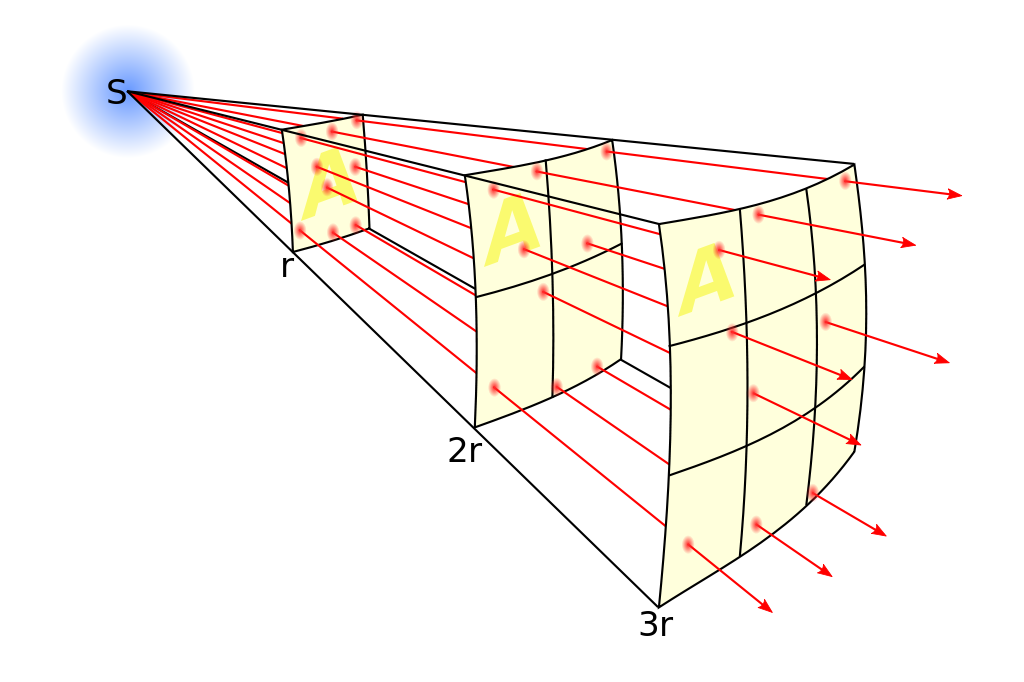
\includegraphics[width=0.4\textwidth]{inversesquare.png}
    \caption{La potencia total en cualquier esfera tiene que ser la misma. \footfullcite{inversesquare}}
  \end{figure}
\end{frame}
%--- Next Frame ---%

\begin{frame}{Densidad de potencia}
  \begin{block}{Definición}
    Definimos la \emph{densidad de potencia} como la cantidad de energía electromagnética que atraviesa una superficie de área A en un determinado tiempo
    \begin{equation}
      p = \frac{\Delta E}{\Delta t A}
    \end{equation}
  \end{block}\pause
  \begin{block}{Observación}
  \begin{itemize}[<+->]
    \item A esta magnitud se la suele llamar \emph{irradiancia} en teledetección.
    \item $[E_\lambda] = W m^{-2} \mu m^{-1}$
  \end{itemize}
  \end{block}
\end{frame}
%--- Next Frame ---%

\begin{frame}{Irradiancia espectral}
  Por ahora venimos trabajando con la densidad de potencia total. Pero uno puede preguntarse cuanta energía llegar de cada longitud de onda en el sol.
  \begin{figure}
    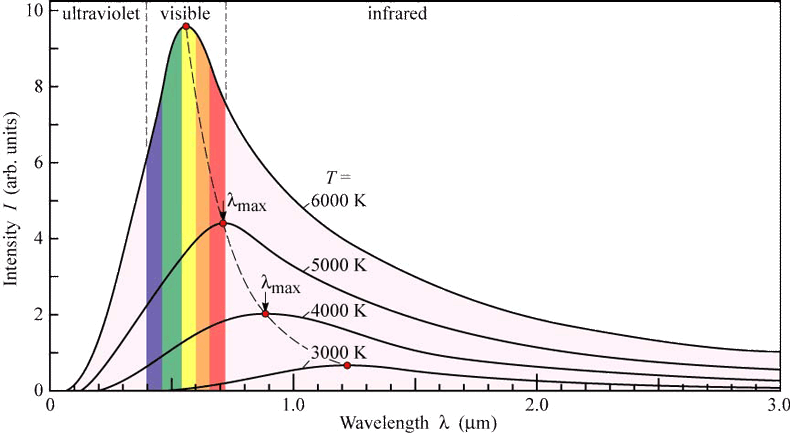
\includegraphics[width=0.8\textwidth]{black-body-radiation-curves.png}
    \caption{Curva de radiancia de un cuerpo negro.}
  \end{figure}
\end{frame}
%--- Next Frame ---%

\begin{frame}{Irradiancia espectral}
  \begin{block}{Radiación de cuerpo negro}
    Para un cuerpo negro ideal
    \begin{equation}
      B(\lambda,T) = \frac{2hc^2}{\lambda^5}\frac{1}{e^{\frac{hc}{\lambda k_B T}}-1}
    \end{equation}
  \end{block}
\end{frame}
%--- Next Frame ---%

\begin{frame}{Irradiancia espectral}
  Si miramos ahora lo que llega a la tierra.
  \begin{figure}
    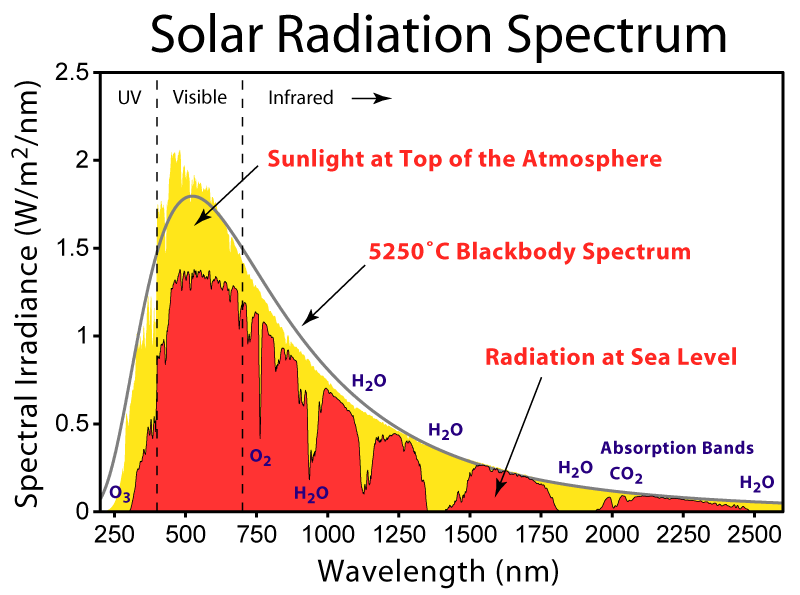
\includegraphics[width=0.6\textwidth]{solar_spectrum.png}
    \caption{Irradiancia solar a tope de la atmósfera.\footfullcite{solar_spectrum}}
  \end{figure}
\end{frame}
%--- Next Frame ---%

\begin{frame}{Irradiancia espectral}
  \begin{exampleblock}{Valores de irradiancia espectral}
    En $[E_{0,i}] = \frac{W}{m^2 \mu m}$
    \begin{figure}
      \begin{tabular}{l c c c}
          Banda & ETM+  & TM    &  OLI \\
          Azul     & 1970  & 1954  & 1925 \\
          Verde     & 1843  & 1826  & 1826 \\
          Rojo     & 1555  & 1558  & 1574 \\
          NIR     & 1047  & 1047  & 955  \\
          SWIR1     & 227.1 & 217.2 & 242 \\
          SWIR2     & 80.53 & 80.29 & 82.5\\
      \end{tabular}
    \end{figure}
  \end{exampleblock}
\end{frame}
%--- Next Frame ---%

\begin{frame}{Irradiancia espectral}
  \begin{block}{Definición}
    Llamamos irradiancia espectral a la distribución de irradiancia en función de la longitud de onda.
  \end{block}
\end{frame}
%--- Next Frame ---%

\begin{frame}{Radiancia}
  El último paso será ver como ver como se comporta la irradiancia en función del ángulo.
  \begin{figure}
    \includegraphics[width=0.4\textwidth]{radiancia.png}
    \caption{Cono de radiación.}
  \end{figure}
\end{frame}
%--- Next Frame ---%

\begin{frame}{Radiancia}
  \begin{block}{Definición}
    La radiancia será la irradiancia por unidad de ángulo solido
    \begin{equation}
      L = \frac{p}{\Delta \Omega \cos\theta_z}
    \end{equation}
  \end{block}
\end{frame}
%--- Next Frame ---%

\begin{frame}{Radiancia}
  \begin{itemize}[<+>]
    \item La irradiancia será lo que medirán los sensores.
    \item Depende del ángulo.
    \item Al igual que la irradiancia tiene nos interesara su dependencia espectral.
    \item $[L_\lambda] = W m^{-2} sr^{-1} \mu m^{-1}$
  \end{itemize}
\end{frame}
%--- Next Frame ---%

\begin{frame}{Radiancia}
  \begin{block}{Definición}
    Llamaremos \emph{radiancia espectral} a la magnitud $L_\lambda$ tal que
    \begin{equation}
      dE = L_{\lambda}(\theta,\phi) \cos(\theta) d\Omega dA dt d\lambda
    \end{equation}
  \end{block}
\end{frame}
%--- Next Frame ---%
\end{document}
